172. \begin{figure}[ht!]
\center{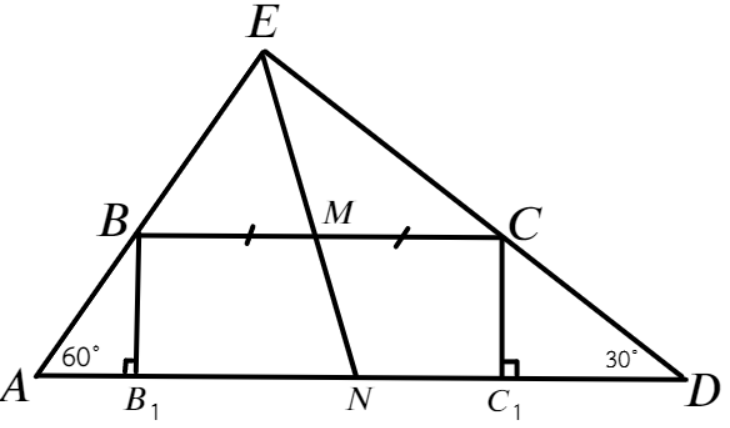
\includegraphics[scale=0.35]{g8-172.png}}
\end{figure}\\
а) Опустим высоты $BB_1$ и $CC_1.$ Пусть высота трапеции равна $x,$ тогда $AB_1=x\ ctg(60^\circ)=\cfrac{\sqrt{3}{3}}x,\ C_1D=x\ ctg(30^\circ)=\sqrt{3}x,$ значит $a=
\cfrac{\sqrt{3}{3}}x+b+\sqrt{3}x,\ \cfrac{4\sqrt{3}}{3}x=a-b,\ x=\cfrac{3(a-b)}{4\sqrt{3}}=\cfrac{\sqrt{3}(a-b)}{4}.$ Тогда
$S_{ABCD}=\cfrac{\sqrt{3}(a-b)}{4}\cdot\cfrac{a+b}{2}=\cfrac{\sqrt{3}(a^2-b^2)}{8}.$\\
б) Продлим боковые стороны трапеции до пересечения, тогда точка их пересечения лежит на одной прямой с серединами оснований (и с точкой пересечения диагоналей, но в нашей задаче это не требуется). Тогда $\angle AED=180^\circ-30^\circ-60^\circ=90^\circ.$ Отрезки $EN$ и $EM$ являются медианами, проведёнными из прямого угла, значит $MN=EN-EM=\cfrac{1}{2}AD-\cfrac{1}{2}BC=\cfrac{1}{2}(AD-BC)=\cfrac{a-b}{2}.$\\
